\subsection{Resultados}
\begin{frame}
    \frametitle{Resultados}
\begin{figure}
\begin{center}
    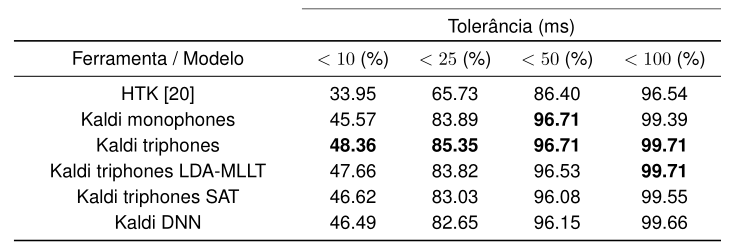
\includegraphics[width=\textwidth]{Figures/table1}
\end{center}
\caption{Distribui��o cumulativa dos limites fon�ticos}
\end{figure}
\end{frame}

\begin{frame}
    \frametitle{Resultados}
\begin{figure}
\begin{center}
    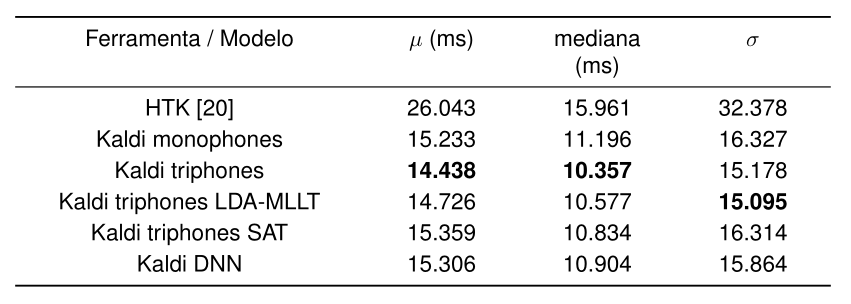
\includegraphics[width=\textwidth]{Figures/table2}
\end{center}
\caption{M�dia, mediana e desvio padr�o dos alinhadores avaliados, em compara��o ao alinhamento manual}
\end{figure}
\end{frame}

\begin{frame}
    \frametitle{Conclus�o}
    \begin{itemize}
        \item Os modelos ac�sticos treinados utilizando o Kaldi obtiveram resultados superiores � outros com suporte � l�ngua portuguesa, e t�o satisfat�rios quanto modelos para outras l�nguas
        \item Foi desenvolvido uma interface para utiliza��o do alinhador
        \item Fatores positivos:
            \begin{itemize}
                \item Avan�os na �rea de reconhecimento de voz para PT-BR
                \item Disponibiliza��o dos recursos desenvolvidos: \url{https://ufpafalabrasil.gitlab.io/}
            \end{itemize}
    \end{itemize}
\end{frame}

% \subsection{Trabalhos Futuros}
% % ----------------------------------------------------------------------------
% \begin{frame}{Trabalhos Futuros}
% \begin{itemize}
% % \item Expandir para outros sistemas operacionais: Windows, MacOS Android
% \item Solu��o alternativa ao \textit{headset}
% \item Sensores alternativos: Microfones de eletreto, BMP180 (press�o)
% \end{itemize}
% \end{frame}
%%% EOF %%%
